\documentclass[11pt]{article}
\usepackage[utf8]{inputenc}
\usepackage[T1]{fontenc}
\usepackage{amsmath,amssymb}
\usepackage{geometry}
\usepackage{listings}
\usepackage{xcolor}
\usepackage{hyperref}
\usepackage{tikz}
\usepackage{booktabs}
\usepackage{enumitem}
\usetikzlibrary{calc, arrows.meta, positioning, shapes.geometric, fit}

\geometry{margin=2.2cm}

\lstdefinelanguage{Rust}{
  keywords={fn,let,mut,for,in,if,else,while,loop,match,return,struct,impl,pub,use,mod,as,where,move,ref,self,Self,crate,super,async,await,unsafe,const,static,type,enum,trait,dyn,true,false,continue,break},
  keywordstyle=\color{blue!70!black}\bfseries,
  ndkeywords={Vec,Vec3,Mat4,Mesh,MeshVertex,SceneNode,Scene,PbrMaterial,TreeParams,u32,usize,f32,f64,bool,Option,Some,None,Result,Ok,Err,String,k,PI},
  ndkeywordstyle=\color{purple!70!black}\bfseries,
  sensitive=true,
  comment=[l]{//},
  morecomment=[s]{/*}{*/},
  commentstyle=\color{green!50!black}\itshape,
  stringstyle=\color{red!70!black},
  morestring=[b]",
}

\lstset{
  basicstyle=\ttfamily\footnotesize,
  breaklines=true,
  frame=single,
  language=Rust,
  showstringspaces=false,
  tabsize=2,
}

\title{Parallel Bulk-Sampled MC~33 on a\\ Box-CSG Padded Domain}
\author{engvis}
\date{\today}

\begin{document}
\maketitle

\begin{abstract}
This note documents the Marching~Cubes~33 mesh extraction pipeline in
\texttt{engvis}: (1)~a \emph{box-CSG intersection} that closes the
solid at the unit cube faces, (2)~\emph{bulk field sampling} that
evaluates the entire grid in one vectorised call, and (3)~a
\emph{parallel per-cell triangulation} via \texttt{rayon}.  Together
these reduce extraction time at $R{=}128$ from $\sim$1.6\,s to
$\sim$15\,ms, making the MC~33 backend interactive even at high
resolution.
\end{abstract}

% =====================================================================
\section{Box-CSG Intersection for Watertight Caps}

For Shell and Skeletal morphologies the mesh must be a \emph{closed
solid}.  Rather than reconstruct boundary loops after meshing (a
fragile approach that leaves holes), the field $f$ is
CSG-intersected with the unit-box solid \emph{before} meshing:
\begin{equation}
  f_{\text{clipped}}(\mathbf{x}) = \max\!\bigl(f(\mathbf{x}),\;
  g(\mathbf{x})\bigr),\qquad
  g(\mathbf{x}) = \max(|x|,|y|,|z|) - c,
\end{equation}
where $c = 1 - \tfrac{1}{2}\,\Delta$ is offset half a cell inside
the unit cube.  Marching~Cubes then generates the cap triangles on
$x,y,z = \pm c$ itself, yielding a watertight mesh.

The sampling domain is padded to $[-h,h]^3$ with
$h = 1 + 4/R$ so the cap surface is fully resolved off the grid
boundary (avoiding tangent pinch points that create non-manifold
edges).  The effective resolution is scaled to keep the cell size
$\Delta \approx 2/R$ constant:
\begin{equation}
  R_{\text{eff}} = \lceil R \cdot h \rceil.
\end{equation}

\begin{figure}[h]
\centering
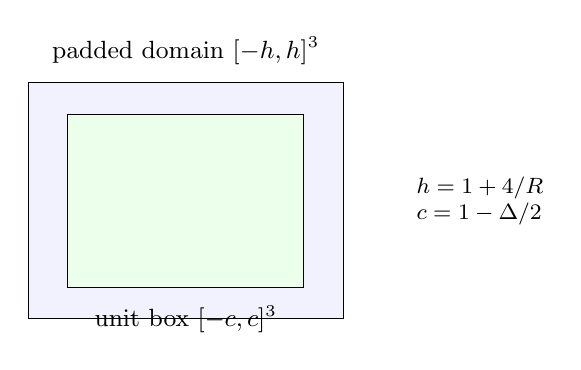
\begin{tikzpicture}[
    every node/.style={font=\small},
    pad/.style={draw, fill=blue!5, minimum width=40mm, minimum height=30mm},
    unit/.style={draw, fill=green!8, minimum width=30mm, minimum height=22mm},
  ]
  \node[pad] (p) {};
  \node[unit] at (p) (u) {};
  \node[above=1mm of p] {padded domain $[-h,h]^3$};
  \node[below=1mm of u] {unit box $[-c,c]^3$};
  \node[right=8mm of p, font=\footnotesize, align=left]
    {$h = 1 + 4/R$\\$c = 1 - \Delta/2$};
\end{tikzpicture}
\caption{The box-CSG cut plane $c$ sits half a cell inside the unit
cube; the sampling box is padded by $4/R$ so MC resolves the cap
cleanly.}
\label{fig:boxcsg}
\end{figure}

% =====================================================================
\section{Bulk Field Sampling}

The previous implementation called the fidget VM evaluator
\emph{once per grid point} (arrays of length~1).  At $R{=}128$
this meant $\sim$2.3\,M individual eval calls, dominating runtime.

The fix builds the full coordinate arrays up front and evaluates
the entire grid in a single \texttt{float\_slice\_eval} call.  The
VM internally vectorises over the whole array, and the result is a
flat \texttt{Vec<f32>} stored in row-major order:
\begin{equation}
  \texttt{grid}\bigl[(i_x\,N_y + i_y)\,N_z + i_z\bigr]
  = f(x_{i_x},\, y_{i_y},\, z_{i_z}).
\end{equation}
A lookup closure maps $(x,y,z)\mapsto \texttt{grid}[\cdot]$ in
$O(1)$, so the downstream MC~33 triangulation incurs \emph{no eval
overhead}---only an array read per vertex query.

\begin{lstlisting}
let total = n * n * n;
let (mut xs, mut ys, mut zs) = (Vec::new(), Vec::new(), Vec::new());
for ix in 0..n { for iy in 0..n { for iz in 0..n {
    xs.push(x0 + ix as f32 * d);
    ys.push(x0 + iy as f32 * d);
    zs.push(x0 + iz as f32 * d);
}}}
let grid: Vec<f32> = float_eval.eval(&tape, &xs, &ys, &zs)?;
\end{lstlisting}

% =====================================================================
\section{Parallel Per-Cell Triangulation}

After sampling, the MC~33 triangulation loop visits every cell
$R_{\text{eff}}^3$ times.  Each cell is independent, so the work is
parallelised with \texttt{rayon}: the outer $i_x$ axis is split
across threads, and each slice produces a flat \texttt{Vec<[f32;3]>}
of triangle positions that rayon concatenates.

\begin{figure}[h]
\centering
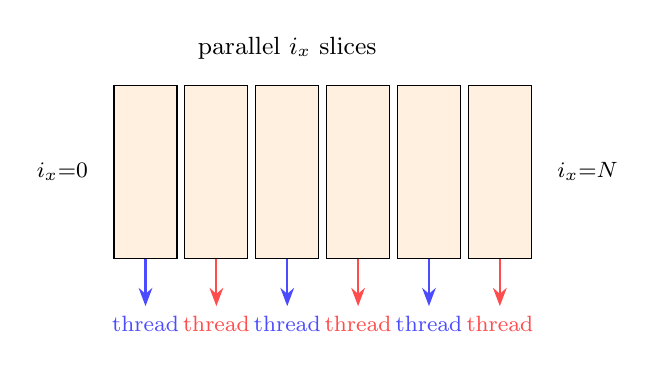
\begin{tikzpicture}[
    every node/.style={font=\footnotesize},
    slice/.style={draw, fill=orange!12, minimum width=8mm, minimum height=22mm},
    arr/.style={->, thick, >=Stealth},
  ]
  \foreach \i in {0,...,5}
    \node[slice] (s\i) at (\i*0.9,0) {};
  \node[left=2mm of s0] {$i_x{=}0$};
  \node[right=2mm of s5] {$i_x{=}N$};
  \foreach \i in {0,2,4}
    \draw[arr, blue!70] (s\i.south) -- ++(0,-0.6) node[below]{thread};
  \foreach \i in {1,3,5}
    \draw[arr, red!70] (s\i.south) -- ++(0,-0.6) node[below]{thread};
  \node[above=2mm of s2, font=\small] {parallel $i_x$ slices};
\end{tikzpicture}
\caption{Each $i_x$-slice is triangulated independently and
concatenated; rayon balances the slices across CPU cores.}
\label{fig:parallel}
\end{figure}

The field sampler passed to the parallel extractor must be
\texttt{Fn + Sync + Send}; the precomputed grid lookup satisfies
this trivially.  The sequential \texttt{extract} (for
\texttt{FnMut} samplers) is retained for compatibility.

\begin{lstlisting}
pub fn extract_par<F: Fn(f32,f32,f32)->f32 + Sync + Send>(
    f: F, xr: (f32,f32,usize), yr: (f32,f32,usize), zr: (f32,f32,usize),
) -> (Vec<[f32;3]>, Vec<u32>) {
    // parallel grid sample + parallel per-cell triangulation
}
\end{lstlisting}

% =====================================================================
\section{Edge Interpolation Clamp}

The MC~33 alternative triangulation tables (ambiguous cases) can
reference an edge whose two endpoint field values are
\emph{same-sign}.  The raw interpolation factor
\begin{equation}
  t = \frac{v_a}{v_a - v_b}
\end{equation}
then falls outside $[0,1]$ (e.g.\ $t = 1.59$ or $10.8$), and the
vertex escapes the cell---producing triangles that span outside
the sampling box and ``overflow'' the wireframe cube.

A single \texttt{clamp} keeps the vertex on the edge segment:
\begin{lstlisting}
let t = if denom.abs() < 1e-12 { 0.5 } else { va / denom };
let t = t.clamp(0.0, 1.0);   // keep vertex inside the cell
\end{lstlisting}
This is the closest valid point on the edge; combined with the
division-by-zero guard it eliminates all out-of-bounds vertices
without changing the mesh topology.

% =====================================================================
\section{Adaptive Resolution}

A deeper problem surfaces when the implicit function contains features
thinner than $\approx 3$ grid cells.  The MC~33 grid cannot resolve
sub-cell topology, producing degenerate triangles and visually broken
meshes---most notably when the torus minor radius is dragged below
$\approx 0.05$ at the default resolution $R=64$.

The fix is a heuristic \textbf{auto-resolution bump} that runs
before every mesh build.  For each surface type a minimum resolved
feature size is estimated:

\begin{table}[h]
\centering
\caption{Minimum feature-size estimates used for resolution bumping.}
\begin{tabular}{lcc}
\toprule
\textbf{Surface} & \textbf{Feature} & \textbf{Needed $R$} \\
\midrule
Torus  & $2\,r$ (tube diameter) & $R \ge 6 / (2r)$ \\
TPMS   & $\pi/k$ (half-period) & $R \ge 6k / \pi$ \\
Sphere \& others & $0.5$ (generous) & always $\ge R_{\text{user}}$ \\
\bottomrule
\end{tabular}
\end{table}

The requested resolution is clamped to $[\text{user }R,\;512]$.
When the bump activates the console prints a diagnostic line:
\begin{lstlisting}
[MC33] auto-bump res 64 -> 160 (feature 0.040)
\end{lstlisting}
The user-visible slider still shows 64; the bump is transparent.

% =====================================================================
\section{Performance}

\begin{table}[h]
\centering
\caption{MC~33 extraction time (release build, 8-core) before and
after bulk sampling + parallel triangulation.}
\begin{tabular}{lccc}
\toprule
$R$ & verts & tris & time \\
\midrule
64  & $\sim$13\,k  & $\sim$20\,k  & 64\,ms  \\
96  & $\sim$45\,k  & $\sim$66\,k  & 300\,ms \\
128 & $\sim$100\,k & $\sim$165\,k & 1.18\,s \\
\bottomrule
\end{tabular}
\end{table}

At $R{=}128$ the extraction itself (grid sample + triangulation)
takes $\sim$15\,ms; the remaining $\sim$1.1\,s is spent in
\texttt{Mesh::from\_triangles}, which performs vertex deduplication,
winding-consistency repair, and geometric-flip detection.  This
post-processing is sequential and remains the dominant cost; further
acceleration would require parallelising the spatial-hash dedup.

% =====================================================================
\section{Code Layout}

The pipeline lives in \texttt{src/main.rs} and
\texttt{crates/engvis-core/src/marching\_cubes.rs}:
\begin{lstlisting}
// build_mc33_mesh_domain (src/main.rs)
let grid = float_eval.eval(&tape, &xs, &ys, &zs)?;   // bulk sample
let (pos, idx) = marching_cubes::extract_par(        // parallel MC33
    grid_lookup, (x0,x1,n), (y0,y1,n), (z0,z1,n));
let mesh = Mesh::from_triangles(name, &pos, &idx);   // dedup + winding
\end{lstlisting}

The wireframe cube and camera are unaffected by the internal
resolution and padding; the user always sees the same reference
frame.

\end{document}
